\chapter{Evaporation: the drying film}
\label{ch:p5}

\begin{keybox}
\textbf{Key idea.} A film is cast from solution and \emph{dries}: solvent
leaves the top surface, the film thins, and the solutes concentrate until
they demix. Evaporation is the \emph{clock} of morphology formation ---
how fast the solvent leaves sets how much time the blend has to phase-
separate before it vitrifies.
\end{keybox}

\section{The model}

We add a moving, evaporating top surface to the ternary system of
Chapter~\ref{ch:p4} (the Landau-mapped moving frame of the
Wodo--Ganapathysubramanian film formulation). The computational box
$[0,1]^2$ represents a physical strip of shrinking height $h(t)$. The
solvent flux at the top drives the frame:
%
\begin{equation}
  K = \sum_i k_{e,i}\,\overline{\phi_i^{\text{top}}} \;\ge 0,
  \qquad \dd{h}{t} = -K ,
\end{equation}
%
and each conserved solute gains a frame-advection term plus a surface-
enrichment flux, arranged so the solute \emph{content} $h\!\int\phi_i$ is
conserved exactly per step (only the solvent leaves). The bulk dynamics
is the ternary Cahn--Hilliard of Chapter~\ref{ch:p4}.

\begin{keybox}
\textbf{The evaporation rate (Biot number).} $k_e$ is the nondimensional
evaporation rate of the solvent --- the Biot number $\mathrm{Bi}=k_e
h_0/D_s$ in the wodo convention. Larger $k_e$ = more volatile solvent =
faster drying. It is \emph{the} processing knob of solution-cast organic
electronics. Different solvents map to different $k_e$; spin speed and
temperature also move it (see the PDPP5T:PCBM Biot values in
\file{materials/materials.yaml}).
\end{keybox}

\section{Run it}

\begin{runbox}
\textbf{Run it.}
\begin{lstlisting}
cd physics/05_evaporation
python run.py            # sweep the evaporation rate
\end{lstlisting}
It dries the same dilute ternary film at several $k_e$ and prints the
drying time, final height, and morphology domain scale. Compare with
\file{EXPECTED.md} and the figures.
\end{runbox}

\paragraph{What you should see.} Every film dries (the mean solvent
fraction $\phi_s$ falls, the height $h$ shrinks), but faster: at
$k_e=\PfiveKeFast$ the film reaches the drying cutoff by $t\approx
\PfiveTdryFast$ (final $\phi_s=\PfivePhisFast$, $h=\PfiveHfast$), while at
$k_e=\PfiveKeSlow$ it lingers to $t\approx\PfiveTdrySlow$. And the
morphology depends on the rate: faster drying freezes a \emph{finer}
pattern (domain scale $\PfiveDomFast$ cells at $k_e=\PfiveKeFast$ vs
$\PfiveDomSlow$ at $k_e=\PfiveKeSlow$) because the blend has less time to
coarsen before it vitrifies.

% --- generated by gen_figures.py ---
\begin{figure}[h]\centering
  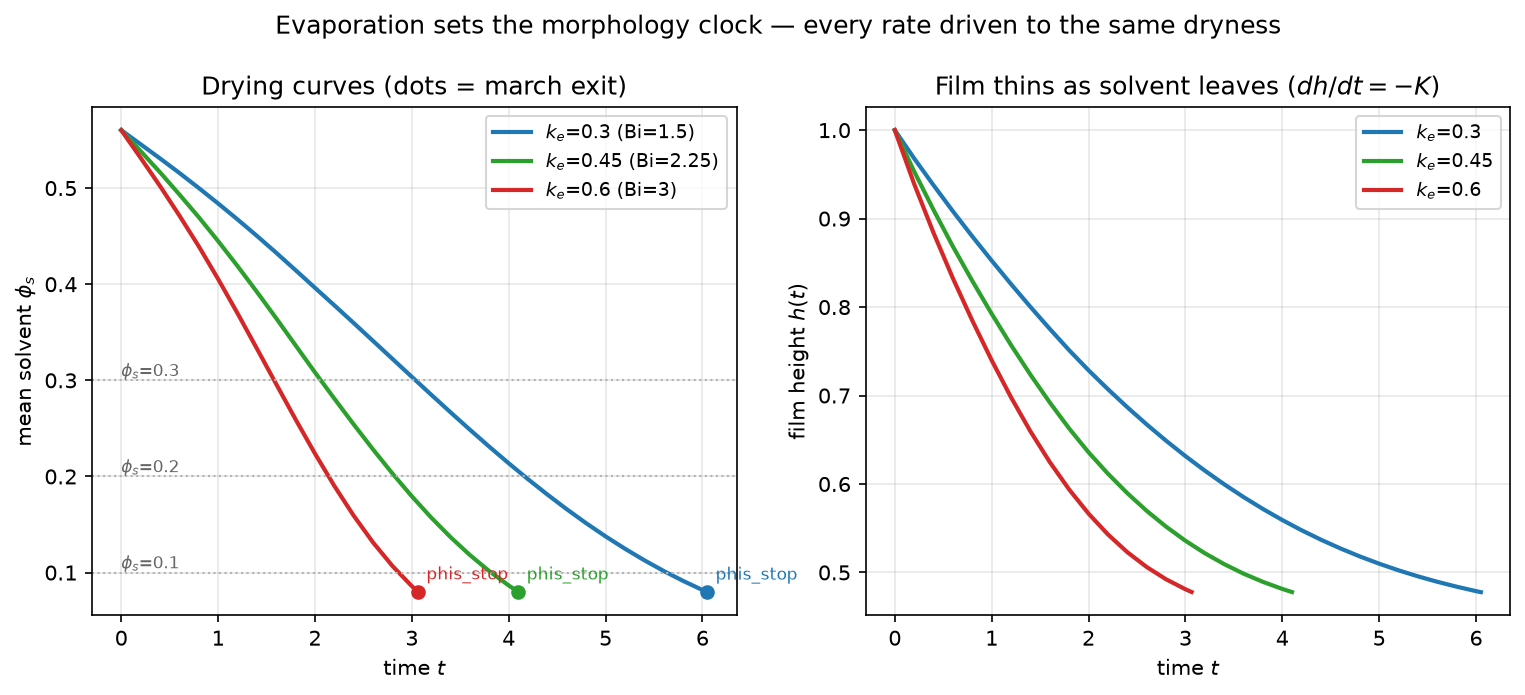
\includegraphics[width=\linewidth]{figures/p5_drying.png}
  \caption{Drying curves (left, mean solvent fraction) and film height
    (right) for several evaporation rates. Larger $k_e$ dries sooner and
    thins faster.}
  \label{fig:p5drying}
\end{figure}

\begin{figure}[h]\centering
  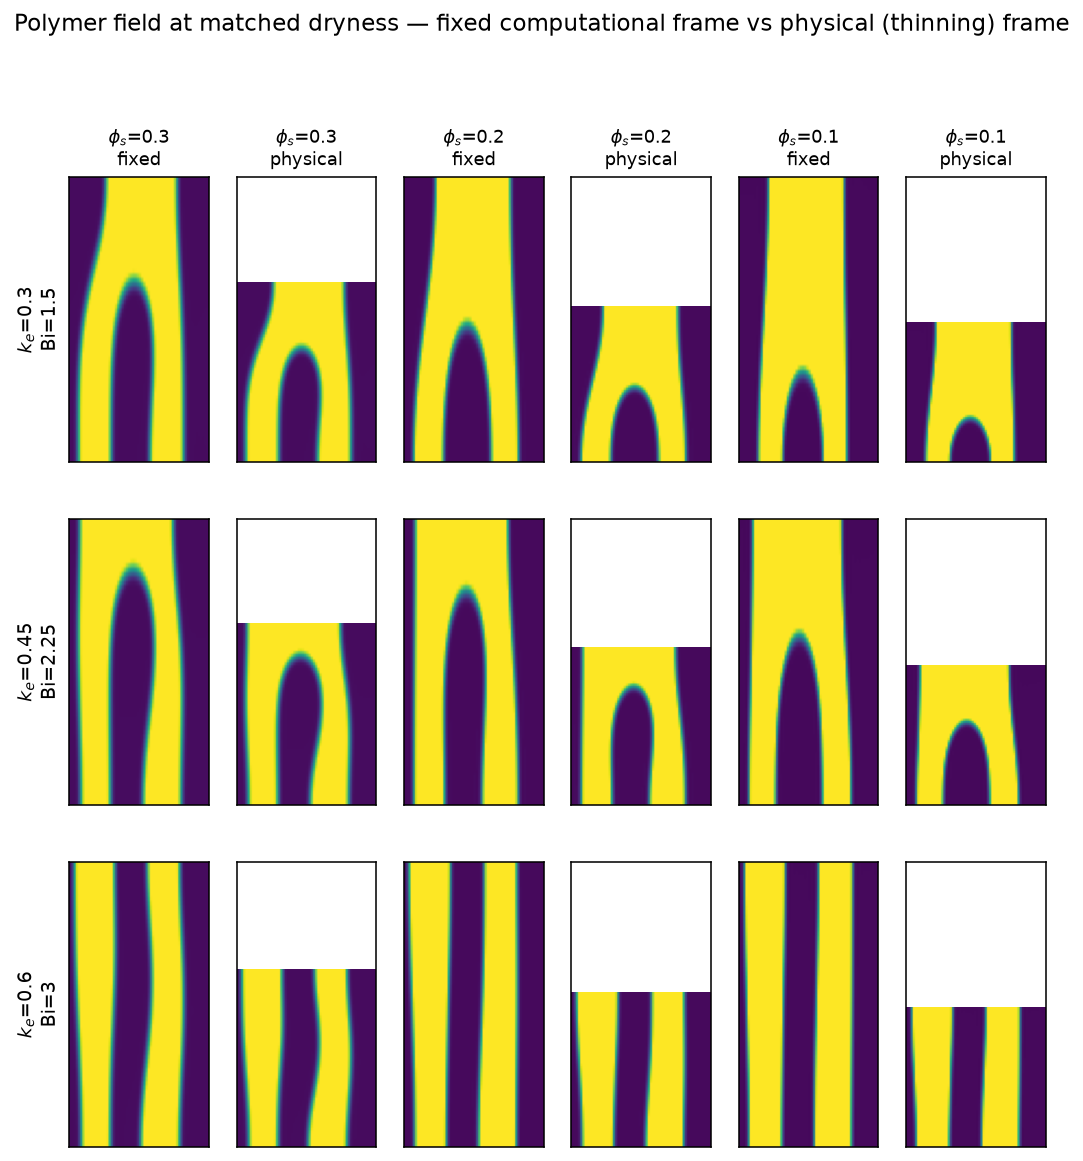
\includegraphics[width=\linewidth]{figures/p5_morphology.png}
  \caption{Dried morphology (the polymer field) vs evaporation rate.
    Faster drying freezes a finer, more kinetically trapped morphology;
    slower drying gives phase separation time to coarsen.}
  \label{fig:p5morph}
\end{figure}

\begin{keybox}
\textbf{Measured self-check.}
\begin{center}\small
\begin{tabular}{lcc}
\toprule
 & slow ($k_e=\PfiveKeSlow$) & fast ($k_e=\PfiveKeFast$) \\
\midrule
drying time $t$        & \PfiveTdrySlow & \PfiveTdryFast \\
final solvent $\phi_s$ & \PfivePhisSlow & \PfivePhisFast \\
final height $h$       & \PfiveHslow & \PfiveHfast \\
domain scale (cells)   & \PfiveDomSlow & \PfiveDomFast \\
\bottomrule
\end{tabular}
\end{center}
\end{keybox}

\section{Code walk-through}

\paragraph{1. Film mode.} A single constructor argument turns on the
moving frame:
\begin{lstlisting}
st = MultiPhaseStepper(dm, M=2, K=0, ..., film=dict(k_e=0.1, h0=1.0))
\end{lstlisting}
\code{k\_e} is the solvent evaporation rate, \code{h0} the initial
height. The stepper carries \code{h\_curr}, updated $-\Delta t\,K$ on each
accepted step.

\paragraph{2. The drying march.} \code{march(..., phis\_stop=0.05,
h\_min=0.15)} adds film stop criteria (dryness / height floor) and the
evaporation $\Delta t$-cap that bounds the height decrement per step.

\paragraph{3. The domain scale.} \code{\_domain\_scale} reads the
characteristic lateral wavelength from the first spectral moment of the
polymer field --- a single number for ``how fine is the morphology''.

\section{Explore on your own}

\question{Push $k_e$ higher and lower by another factor. Does the domain
scale keep shrinking with rate, or does it saturate? What sets the
finest morphology you can freeze in?}

\question{Change the solvent selectivity ($\chi_{1s}$ vs $\chi_{2s}$).
Does a solvent that likes one solute more change which component
enriches at the drying surface?}

\question{The drying curve $\phi_s(t)$ is roughly linear early
(constant-rate period) then bends. Explain the bend in terms of the
surface composition feeding back into $K=\sum_i k_{e,i}
\overline{\phi_i^{\text{top}}}$.}

\question{Combine this with Chapter~\ref{ch:p3}: add a substrate wall
energy and dry the film. Does evaporation-driven enrichment at the top
compete with substrate enrichment at the bottom? Which wins?}

\question{Two solvents of different volatility can be modelled as
different $k_e$. Predict how a fast vs a slow solvent changes the
vertical stratification, then test it.}

% ====================================================================
